%========================================================================================================================
%========================================================================================================================
%========================================================================================================================
\section{Semantics}
\label{sec:semantics}
In this section, we present the consistency enforcement mechanism of
\tool, abstracted as a formal operational semantics. Our approach is
complete for the specification language defined in
Sec.\ref{sec:ctrt_language}, however for better
comprehensibility, here we present the semantics and the theorems
paramterized over a non-hybrid contract consisting of a single  proposition.
Therefore, in the rest of this section, we will assume a given contracat $\psi$
of the following form:
\begin{fmathpar}\footnotesize
\begin{array}{lll}
\psi = \forall a. a \xrightarrow{\rel_1;\rel_2;...;\rel_k} \hat{\eta} \Rightarrow a 
\xrightarrow{\visZ} \hat{\eta}
&\qquad 
\quad & \rel_i \in \{\visZ;\soZ\}
\end{array}
\end{fmathpar}
%
%

The operational semantics defines a small-step relation over \emph{execution
states}, which are tuples of the form {\footnotesize $\E=(\EffSoup,\visZ
,\soZ)$}.
The \emph{effect soup} $\EffSoup$, stands for the set of all
effects produced in the system, and \emph{primitive relations}
{$\visZ,
\soZ \subseteq \EffSoup \times \EffSoup$}, respectively represent the
visibility and session order 
among such effects. Figures \ref{subfig:execution_graph} and
\ref{subfig:execution_example} present a simple
execution state consisting of 9 effects with associated
primitive relations\footnote{we omit drawing transitive $\soZ$
edges (e.g. between
$\eff_8$ and $\eff_1$) for better readability}.
\begin{figure}[h]
	
	\begin{subfigure}[b]{0.28 \textwidth}
	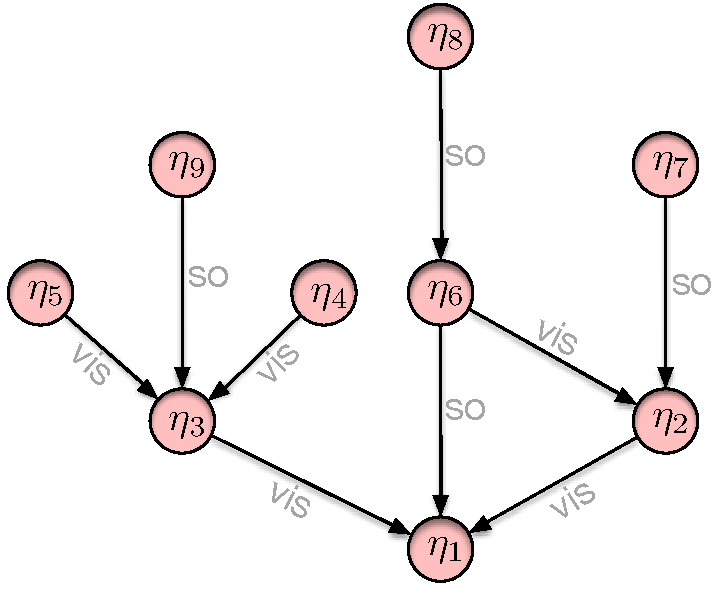
\includegraphics[scale=0.38]{Figures/execution.pdf}
	\subcaption{An execution state \E}
	\label{subfig:execution_graph}
	\end{subfigure}
	%
	\quad \vrule \quad
	%
	\begin{subfigure}[b]{0.31 \textwidth}
	\begin{smathpar}
	\begin{array}{lcl}
	\E.\EffSoup & = & 
	\{\eta_1,\eta_2,\eta_3,\eta_4,\eta_5,\eta_6,\eta_7,\\ & & \;\eta_8,\eta_9\}\\
	\E.\visZ & = & 
	\{(\eta_5,\eta_3),(\eta_4,\eta_3),(\eta_3,\eta_1),\\ &
	&\;(\eta_2,\eta_1),(\eta_6,\eta_2)\} \\ 
	\E.\soZ & = & \{(\eta_9,\eta_3),(\eta_8,\eta_6),(\eta_6,\eta_1),\\ 
	& & \;(\eta_8,\eta_1),(\eta_7,\eta_2) \} \\ 
	\end{array}
	\end{smathpar}\\
	\subcaption{Effect soup and primitive relations}
	\label{subfig:execution_example}
	\end{subfigure}
	%
	\quad \vrule \quad
	%
	\begin{subfigure}[b]{0.3 \textwidth}
	\begin{smathpar}
	\begin{array}{lll}
	\visZ^{-1}  (\eta_1) & = & \{\eta_2,\eta_3\} \\ 
	\soZ^{-1}  (\eta_1) & = & \{\eta_6, \eta_8\} \\
	(\soZ\cup\visZ)^{-1} (\eta_1) & = &
	\{\eta_2,\eta_3,\eta_6,\eta_8\} \\ 
	(\visZ^*)^{-1} (\eta_1) & = &
	\{\eta_2,\eta_3,\eta_4,\eta_5,\eta_6\} \\ 
	(\soZ;\visZ)^{-1}(\eta_1) & = & \{\eta_7,\eta_9\}
	\\ \\
	\end{array}
	\end{smathpar} \\
	\subcaption{Relation inverse examples}
	\label{subfig:inverse_example}
	\end{subfigure}
	\caption{A simple execution state }
\label{fig:execution_state}
\end{figure}

We denote the subset of $\EffSoup$ consisting of effects that
satisfy a certain condition as $\EffSoup_{(\mathtt{condition})}$.

% models
Note that \tool's contracts are in fact constraints over execution states,
where the domain of quantification is fixed to the effect soup
$\EffSoup$, and
interpretation for $\soZ$ and $\visZ$ relations (which occur free in the
contract formulae) are also provided. Thus, execution states are
potential models for any first-order formula expressable in the
specification language. If an execution state $\E$ is in fact a valid model
for a contract $\psi$, we say that $\E$ satisfies $\psi$, written as $\E
\models \psi$. 

%reduction relation
The reduction relation in our semantics is of the form
{\footnotesize $
(\E,\op_{<s,i>}) \;\xrightarrow{V}\; (\E', \eff),
$}
which can be interpreted as the transformation of the initial execution state
$\E$, caused by a replica with a local 
set of effects $V$, when it executes
$\op$, the $i^{th}$ operation from the session $s$. 
During this reduction step, a new effect $\eff$ is produced and added to
the system, resulting in a new execution state $\E'$ composed of an updated effect
soup and new primitive relations.





%=============================================================================================================
%=============================================================================================================
%--------- Definitions to be used in the semantics
%=============================================================================================================
\subsection{Preliminaries}
\label{subsec:prelim}
In this part, we will present the formal definitions and notations
required to explain our operational semantics.
We start by defining the interpretation of an \emph{inversed} 
dependency relation 
{\footnotesize $\Rel^{-1}$} under an execution state $\E$, 
which is utilized in the basis of our consistency enforcement mechanism.
We previously mentioned our interpretation for $\soZ$ and $\visZ$
between
effects under  $\E$, which can now be straightforwardly extended to their inverse as
follows\footnote{Note that when the input of an inversed relation is a singleton
$\{\eta\}$, we drop the brackets and simply write it as
$\rel^{-1}(\eta)$}:
\begin{equation}
\label{eq:r_inv}
\scriptsize
\rel^{-1}(S) = 
\begin{array}{lcl}
\bigcup\limits_{b\in S}\{a|(a,b) \in \E.\rel \} & \qquad & \rel\in\{\soZ,\visZ\}
\end{array}
\end{equation}
Additionally, based on our interpretation of the sequences of seed
relations given in Sec.\ref{sec:ctrt_language}, we can
extend the above definition to the following:
\begin{equation}
\label{eq:seq_inv}
\scriptsize
\begin{array}{lllll}
b \in  (\Rel';\rel)^{-1}(a) & \iff & \exists c. c \in \rel^{-1}(a)
& \wedge & b \in (\Rel')^{-1}(c) 
\end{array}
\end{equation}
Now, It might seem that we are ready to define any $\Rel^{-1}$ 
based on  the two definitions above; 
however, note that definition (\ref{eq:seq_inv}) fails to capture
the reality of our system model, where all computations are
performed by replicas independently, which at any given moment, might have access to only a
\emph{subset of all produced effects} in the system.
For example, consider  {\footnotesize$(\soZ;\visZ)^{-1}(\eta_1)$} under the
execution state presented in Fig.\ref{fig:execution_state}. 
In order to compute this set, based on (\ref{eq:seq_inv}) we have: 
\begin{smathpar}
\scriptsize
\begin{array}{lllll}
b \in  (\soZ;\visZ)^{-1}(\eta_1) & \iff & \exists c. c \in
\visZ^{-1}(\eta_1)
& \wedge & b \in (\soZ)^{-1}(c)
\end{array}
\end{smathpar}
Now, since there exist \emph{mid-level} effects $c=\eta_2$ and 
$c=\eta_3$, such that satisfy the above definition respectively 
for $\eta_7$ and $\eta_9$, we can conclude: {\footnotesize$(\soZ;\visZ)^{-1}(\eta_1) =
\{\eta_7,\eta_9\}$}.
Now consider a replica that contains {\footnotesize$\{\eta_1, \eta_6, \eta_7,
\eta_9\}$} at the moment, and wants to check if the dependencies of $\eta_1$ are locally present 
or not. Even though based on the above definition, the
answer is affirmativ (since the replica does contain $\{\eta_7,\eta_9\}$), but in
reality the replica has no way of verifying it, since the mid-level
effects $\eta_2$ and $\eta_3$ are not present at the replica yet. 

To capture the above property, we now partially define the 
inverse of $\Rel$, \emph{according to a set of available effects $V$}, 
only if all the required mid-level effects are present in $V$.
The following is our definition, based on (\ref{eq:r_inv}) and a more
strict version of (\ref{eq:seq_inv}):
\begin{equation}
\label{eq:R_inv}
\scriptsize
b \in \Rel^{-1}_V(a) \iff
\begin{cases}
\begin{array} {lllll} 
\bot & \;\myif\; & \Rel = \nullR& & \\
b \in \rel^{-1}(a) & \;\myif\; & \Rel=\rel & & \\
\exists c. c \in
\rel^{-1}(a) \wedge b \in (\Rel')_V^{-1}(c) \wedge
\rel^{-1}(a) \subseteq V   & \;\myif\; & \Rel=\Rel';\rel & & \;
\end{array}
\end{cases}
\end{equation}
For example, in Fig.\ref{fig:execution_state}, 
{\footnotesize  ($\eta_9 \in
(\soZ;\visZ)_{\{\eta_1,\eta_3\}}^{-1}(\eta_1)$)}
holds, but {\footnotesize($\eta_9 \not\in (\soZ;\visZ)_{\{\eta_1\}}^{-1}(\eta_1)$)}. 
Furthermore, we can now define a set $V$ to be \emph{self-contained} for
a given effect $\eta$,
written as {\footnotesize $\SC
R \eta V$}, if $V$ contains all the required mid-level effects to compute
$R$ inverse of $\eta$ in totality, i.e.
\begin{equation}
\scriptsize 
\SC R \eta {V} \iff R^{-1}_V(\eta) = R^{-1}_{E.A}(\eta)
\end{equation}
For example in Fig.\ref{fig:execution_state}, {\footnotesize $\SC R
{\eta_1} V$} holds for an arbitrary  $R$ and for any $V$ that is a superset of
{\footnotesize $\{\eta_1,\eta_2,\eta_3,\eta_4,\eta_5\}$}.

Now, we define {\footnotesize \trunc{}} as a function that
given  $R \in$ \relationS{}, 
returns a new relation by removing the last element from the sequence
in R:
\begin{equation}
\scriptsize
\trunc{R} = 
\begin{cases}
\begin{array}{lcl}
\nullR & \quad \myif \quad & R = \rel \quad \mathtt{or} \quad R = \nullR \\
R' & \quad \myif \quad & R = R';\rel 
\end{array}
\end{cases}
\end{equation}

Finally, we define \emph{closed subsets} of a given set $V$, 
as the subsets that are closed under {\footnotesize$(\trunc{R}^{-1}_V)$}, that
also contain all the required mid-level effects to compute
{\footnotesize $\trunc{R}^{-1}$}.
Moreover, we define the largest element among such
subsets, as the \emph{maximally closed subset} of V as follows\footnote{We slightly abuse the previously defined notation
in (\ref{eq:R_inv})
and use a \emph{set} of effects as the input of
$R^{-1}$, which is defined as:
$x \in R^{-1}_V(S) \iff \exists (y\in S). x \in R^{-1}_V(y)$}:
%
\begin{fmathpar}
\begin{array}{rlllll}
\mathtt{closed \; subsets:} &  V' \in \left \lfloor  V \right \rfloor & \iff & V' \subseteq V & \wedge &
(\trunc R)_V^{-1}(V') \subseteq V' ~\wedge ~ \SC {\trunc{R}} \eta {V'}    \\
\mathtt{maximally \; closed \; subset:} & V' = \left \lfloor  V \right
\rfloor_{\mathtt{max}} & \iff & V' \in \left \lfloor  V \right \rfloor &
\wedge & \not\exists V'' \in \left \lfloor  V \right \rfloor. |V''|>|V'|
\end{array}
\end{fmathpar}






%=============================================================================================================
%--------- The operational semantics
%=============================================================================================================
\subsection{Core Operational Semantics}

\begin{figure}[t]
\raggedright
\textbf{Auxiliary Definitions}\\ \vspace{-2mm}
%
\begin{minipage}{0.5\textwidth}
\begin{fmathpar}
\begin{array}{lclcl}
  \multicolumn{5}{c}{
    {op} \in \mathtt{Operation\; Name} \spc \spc
    {v} \in \mathtt{Return\; Value} \spc \spc
    {s} \in \mathtt{Session\; Id} \spc\spc
  } 
  \\ 
  \eff & \in & \mathtt{Effect} & \coloneqq &  (s,op,v)\\
  F_{op} & \in & \mathtt{Op.\,Def.} & \coloneqq & \set{\eff} \mapsto v\\
  \EffSoup & \in & \mathtt{Eff\,Soup}	  & \coloneqq & \set{\eff} \\
  \visZ,\soZ &	\in & \mathtt{Relations} & \coloneqq & \set{(\eff,\eff)} \\
  {\E} 	& \in & \mathtt{Exec\;State}  & \coloneqq & \Exec \\
\end{array}
\end{fmathpar}
\end{minipage}
%

\vspace {3mm}

\textbf{Auxiliary Reduction} \; \\
\fcolorbox{black}{pgrey}{\scriptsize \(\auxred{S} {(\E,op_{<s,i>})} {} {(\E',\eff)}\)}\\
\begin{minipage}{0.9\textwidth}
\vspace{2mm}
\rulelabel{Oper}
\vspace{-2mm}
\begin{fmathpar}
\stretcharraybig
\begin{array}{l}
\RuleTwo
{
%\Theta(\rho \mapsto (v,cache)) \qquad
S \subseteq \EffSoup \qquad F_{op}(S) = v \qquad
\eta \not\in S \qquad
\eff = (s,op,v) \qquad  \\
%\id(\eta) = i \qquad
%\{\eff'\} = \EffSoup_{({\sf SessID}=s,\,{\sf SeqNo}=i-1)}\\
\EffSoup' = \EffSoup \cup \{\eff\}  \qquad
\visZ' = \visZ \cup S \times\{\eff\}\qquad
\soZ' = \soZ \cup \{(\eta',\eta) \,|\, \eta'\in \EffSoup_{({\sf
SessID}=s)}      \}\qquad
%\soZ' = (\soZ^{-1}(\eff') \cup \eff') \times\{\eff\} \cup \soZ
}
{
  \auxred {S} {((\EffSoup,\visZ,\soZ), op_{<s,i>}))}
  {} {((\EffSoup',\visZ',\soZ'),\eta)}
}
\end{array}
\end{fmathpar}
\end{minipage}
\vspace{4mm}\\
\textbf{Operational Semantics} \; \\
  \fcolorbox{black}{pgrey}{\scriptsize \((\E,op_{<s,i>}) \;\xrightarrow{V}\; (\E',\eff)\)}\\
\vspace{2mm}
\begin{minipage}{0.45\textwidth}
\rulelabel{UB Exec}
\vspace{-2mm}
\begin{fmathpar}
\stretcharraybig
\begin{array}{l}
\RuleTwo
{
  \visZ \subseteq r_k \spc
  V \subseteq E.A \spc  
  V'= \left \lfloor V \right \rfloor_V \spc
  \\ %   R^{-1}_{V}(\eta) \subseteq V' \\
  \auxred {V'} {(E, op_{<s,i>}))}
    {} {(E',\eta)} 
}
{
  (\E,op_{<s,i>}) \;\xrightarrow{V}\; (\E', \eff)
}
\end{array}
\end{fmathpar}
\end{minipage}
\hfill
\begin{minipage}{0.45\textwidth}
\rulelabel{LB Exec}
\vspace{-2mm}
\begin{fmathpar}
\stretcharraybig
\begin{array}{l}
\RuleTwo
{
     \visZ \not\subseteq r_k \spc
     V \subseteq E.A \spc  
     R^{-1}_{V}(\eta) \subseteq V \\
  \auxred {V} {(E, op_{<s,i>}))}
    {} {(E',\eta)} 
}
{
  (\E,op_{<s,i>}) \;\xrightarrow{V}\; (\E', \eff)
}
\end{array}
\end{fmathpar}
\end{minipage}
\\
\vspace{5mm}
\hrulefill\\
\caption{Core Operational semantics of a replicated data store.}
\label{fig:semantics}
\end{figure}

 %--- The Figure Containing the Rules
%--- Section intro
In this part we present the operational semantics, as a set of rules representing our
consistency enforcement approach.
Fig.\ref{fig:semantics} presents the rules defining the
auxiliary relation ($\hookrightarrow$) and then the small-step reduction relation 
($\rightarrow$) over execution states, where the latter is parametrized
over a set $V$,
which stands for the locally available set of effects at the replica
taking the reduction step. 
Trivially, $V$ must be a subset of all effects in the system at the
initial execution state, however, there is no other restrictions on $V$,
since we only assume eventual consistency at the underlying store.

%--- The Aux [OPER] rule
The rule
\rulelabel{oper} defines the abstract procedure of generating a new effect $\eff$, by witnessing a set
of effects $S$, using a user-defined function $F_{op}$. 
We formally define an effect as a tuple $\eff=(s,op,v)$, representing the
session and the operation name 
whose execution created $\eff$, and the value $v$
that the replica returns, responding to that operation.
%
Moreover, the rule explains how the execution state changes after a new
effect is produced. Specifially, in the new execution state, 
the effect soup
$\EffSoup'$ contains the newly created effect $\eff$,
the relation $\visZ'$
captures the fact that all effects in the set $S$ were made
visible to $\eta$, and $\soZ'$ states that all effects from the same
session as the current operation, that are
already presenet in the system, should be in session
order with $\eff$ in the final execution state.

%--- rule for (->) relation
%UB
Now we explain the rules for the reduction relation $(\xrightarrow{V})$,
starting with \rulelabel{ub exec}, 
which defines the execution of an
operation in a replica under a \UB{} contract. 
The rule requires operations to only witness $V'$, the maximally closed
subset of $V$, or in other words, the rule governs replicas to 
create safe environments for operations, by
filtering out effects that may cause the specified anomaly. 

%LB
The next rule, \rulelabel{lb exec}, defines the step taken by a
replica, when an
operation is executed under an \LB{} contract. The precondition 
$R_V^{-1}(\eff)\subseteq V$ in the rule, ensures that the reduction
happens only if the effects necessary to avoid the specified anomaly are
present in V, assuming that V contains all the mid-level effects to
determine dependencies of the newly created effect $\eta$ (i.e.
is a self contained set). In other words, the rule governs replicas to
block execution of an operation under an \LB{} contract, if the replica is unable to verify the
presence of all necessary dependent effects.


%=============================================================================================================
%--------- Theorem on correctness of enforcement
%=============================================================================================================
\subsection{Soundness and Optimality}
\label{subsec:sound}
%
%Subsection on the correctness of contract 
%
In order to prove a meta-theoretic correctness property for our
semantics, we first define a $\psi$-consistent set of effects $S$ given
a execution state $\E$ as follows:

\begin{equation}
\scriptsize
S \mathtt{\;is\;} \psi \mathtt{-consistent} \iff \forall (\eff \in S).
\forall(a\in \E.\EffSoup). \trunc{R}(a,\eta)
\Rightarrow a \in S
\end{equation}
%Where the definition of $R$ is based on the definition of $R^{-1}$ from
%subsection 
%\ref{subsec:prelim}:
%\begin{equation}
%\scriptsize
%R(a,b) \iff a \in R_{E.A}^{-1}(b)  
%\end{equation}
\begin{theorem}
\label{theorem:one}
For all reduction steps 
$
\scriptsize
\; (\E,op_{<s,i>}) 
    \xrightarrow{V}
  (\E',\eff)  
$,
\begin{fmathpar}
\begin{array}{ll}
(i) & \mathtt{if\;} V \mathtt{\;is\;} \psi \mathtt{-consistent\;} \mathtt{under\;} \E,
\mathtt{\;then\;}  V \cup \{\eta\} \mathtt{\;is\;} \psi\mathtt{-consistent \; under\;} E'  \\
(ii) & E' \models \psi[\eta/\hat{\eta}]
\end{array}
\end{fmathpar}



\end{theorem}
\begin{proof}
Appendix \ref{app:proof1}
\end{proof}







%=============================================================================================================
%--------- Theorem on maxVis and minWait
%=============================================================================================================
%
%Subsection of the maximality of the set made visible and liveness
%properties 
%
\begin{theorem}
\label{theorem:two}
For all reduction steps
{\footnotesize $
(\E,op_{<s,i>}) 
    \xrightarrow{V}
  (\E',\eff) 
$},
the set of effects made visible to $\eta$ is maximal. i.e. for all
 {\footnotesize $a \in V$}, if 
 {\footnotesize $ \SC {\trunc{R}} a V$}, then 
\begin{fmathpar}
(a,\eta) \not\in \E'.\visZ \Rightarrow 
(\E'.A,\E'.\visZ \cup \{a,\eta\}, \E'.so) \not\models \psi[\eta/\hat{\eta}]
\end{fmathpar}
\end{theorem}


%
% THE MINIIMAL WAIT THEOREM
%

\begin{theorem}
\label{theorem:three}
For all execution states $E$, if there
exists ($S\subseteq E.A$) such that: 
\begin{smathpar}
\auxred{S} {(\E,op_{<s,i>})} {} {(\E',\eff)} \spc \wedge \spc (\mathtt{S \cup \{\eta\} \; is 
\;} \psi \mathtt{-consistent \; under \;} E' )  
\end{smathpar}
then there exist  $E''$, $\eff'$ and $V\subseteq E.A$ such that:
$((\E,op_{<s,i>})\;\xrightarrow{V}\;(\E'',\eff'))$
\end{theorem}
\begin{proof}
The proof is given by choosing set $V$ to be equal to $S$, and then
considering two cases, where either $S$ or $\left \lfloor S \right
\rfloor_S$ are made visible to operations, if the contract is respectively
waiting and non-waiting. In both cases, all premises of taking an step
are satisfied.
A detailed proof can be found in appendix
\ref{app:proof3}.
\\
\end{proof}


























% GENERALIZATION OF THE SEMANTICS WHICH I DONT THINK SHOULD BE INCLUDED
% BECAUSE OF LACK OF SPACE
%=============================================================================================================
%=============================================================================================================
\begin{comment}
%=============================================================================================================
%--------- How it can be generalized for all contracts
%=============================================================================================================
\subsection{Generalization}
\label{subsec:generalization}
We finish this section by extendeding our ideas in two dimentions. 
We will first explain how to handle an arbitrary
contract $\psi$ of the following form:  
\begin{fmathpar}
\psi = \pi_1 \wedge \pi_2 \wedge ... \wedge \pi_m \qquad \qquad 
\pi_i = \forall (a,b). a \xrightarrow{R_i} b \Rightarrow a
\xrightarrow{\visZ} b
\end{fmathpar}
Later, we will
explain how to maintain multiple levels of consistency simultaneously,
each of which is defined for a different operation name. We will assume an arbitrary contract
$\psi_{\op}$ for every user-defined operation $\op$, and explain how to
modify our system model to preserve them all.

To begin with, as we mentioned earlier, all propositions in our specification language,
either put a maximal or a minimal bound on the subset of local effects 
to be made visibe to each opreation. 
This simply means that when the system is given a conjunction
of propositions, it should define the such subsets in a way, so it would not violate
\emph{any} of them. 
Therefore, by a few modifications we can extend the system to support
all contracts. Firstly, the single premise $R_V^{-1}(\eta) \subseteq V$
in the reduction rule should be replaced with the following
conjunction: 
\begin{fmathpar}
\bigwedge_{1 \leq i \leq m} (R_i)_V^{-1}\subseteq V
\end{fmathpar}
Secondly, the definition of the maximal closed subset of local effects
must also be modified to a subset that is closed under \emph{all} given
relations:
%---------------------------------------------------------------------
% I am not sure if we should include the formal definition here. It is
% unnecessarily complex
\begin{fmathpar}
\left \lfloor S \right \rfloor_V = S' \spc \iff \spc S'
\subseteq S \; \wedge \;
\bigwedge(R_i)_V^{-1}(S') \subseteq S' \; \wedge \; 
\not\exists
S''.(\bigwedge ((R_i)_V^{-1}(S''))\subseteq S''\wedge |S''|>|S'|)
\end{fmathpar}
%---------------------------------------------------------------------

Moreover, for modifying the system to handle multiple contracts
simultaneously, we can
extend the local effect set $V$, to a sequence
of sets $V_{\op_i}$, each maintaning  the consistency level for an
operation type $\op_i$. Now we define the modified form of execution steps as
follow:
\begin{fmathpar}
(\E,\op_{<s,i>}) 
    \;\xrightarrow{V_{\op}}\;
  (\E',\eff) 
\end{fmathpar}
The local effect set $V$ must also be replaced with $V_{\op_i}$ in the 
premises of the reduction rules, so each operation of type $\op_i$ would
only witness the associated subset for its own consistency requirements.
This abstractly represents our implementation, in the sense that all operations
work only on a specific subset of available effects at any replica. The subset, is
maintained according to the contract assosiated with each operation, and
is guaranteed to preserve the consistency requirements following the
theorems of sections \ref{subsec:sound} and \ref{subsec:opt}. 
\end{comment}
